\documentclass[11pt,letterpaper]{article}
\usepackage{style}

%% ------- INICIA DOCUMENTO ------
\begin{document}
\begin{titlepage}
\begin{center}
\begin{LARGE}
INSTITUTO POLITÉCNICO NACIONAL\\
\vspace*{0.15in}
ESCUELA SUPERIOR DE CÓMPUTO\\
\end{LARGE}
\vspace*{1.0in}
\begin{Large}
%% NOMBRE DE LA PRÁCTICA O EXAMEN
\textbf{TÉCNICAS DE CRUZA 1} \\  
\end{Large}
\vspace*{0.2in}
\begin{large}
\textit{Práctica 6}\\
\end{large}
\vspace*{1.0in}
\begin{large}
%% INTEGRANTES	
Dominguez de la Rosa Bryan\\
\vspace*{2.0in}
GRUPO 3CM5\\
\vspace*{0.2in}
Profesor: Morales Güitron Sandra Luz\\
\vspace*{1.5in}
\today
\vspace*{0.3in}
\end{large}
\rule{150mm}{0.1mm}\\

\end{center}
\end{titlepage}

%% --------- COMIENZA EL DESARROLLO DEL DOCUMENTO --------

\section*{Introducción}
El Centro de Investigación en Computación (CIC) es un organismo de excelencia en Ciencias de la Computación e Ingeniería de Cómputo, cuyo objetivo es realizar investigación científica de vanguardia orientada a la enseñanza en el posgrado, a la investigación básica y aplicada,así como al desarrollo tecnológico.\\

La exposición de las áreas de investigación estaban divididas por los distintos laboratorios que existen en el Centro; a continuación se presenta descripción de los proyectos observados.


\subsection*{Sistemas Inteligentes para la Automatización}

El proyecto presentado se trataba de un sistema que permitía la detección de sismos en la Ciudad de México, a través de una red de sensores que se colocan en puntos estratégicos de los edificios. Se conectan a través de enrutadores para generar la comunicación entre sensores. En el software se observa el análisis de la señal generada, así como unas representaciones de las posibles inclinaciones de detectables de edificios, simuladas por computadora.

\begin{figure}[H]
	\centering
	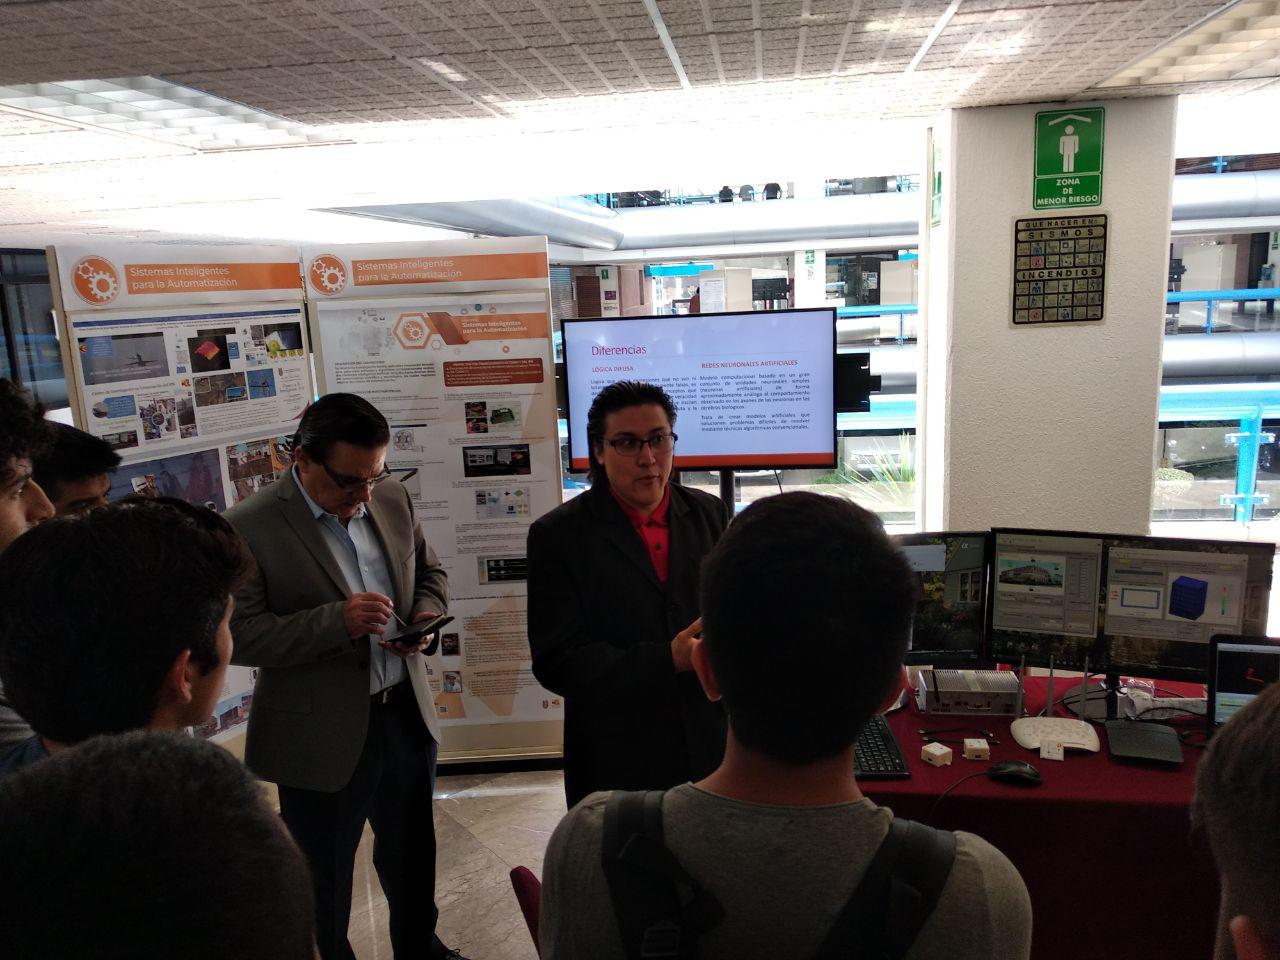
\includegraphics[scale = 0.4]{images/sismo1}
\end{figure}

\begin{figure}[H]
	\centering
	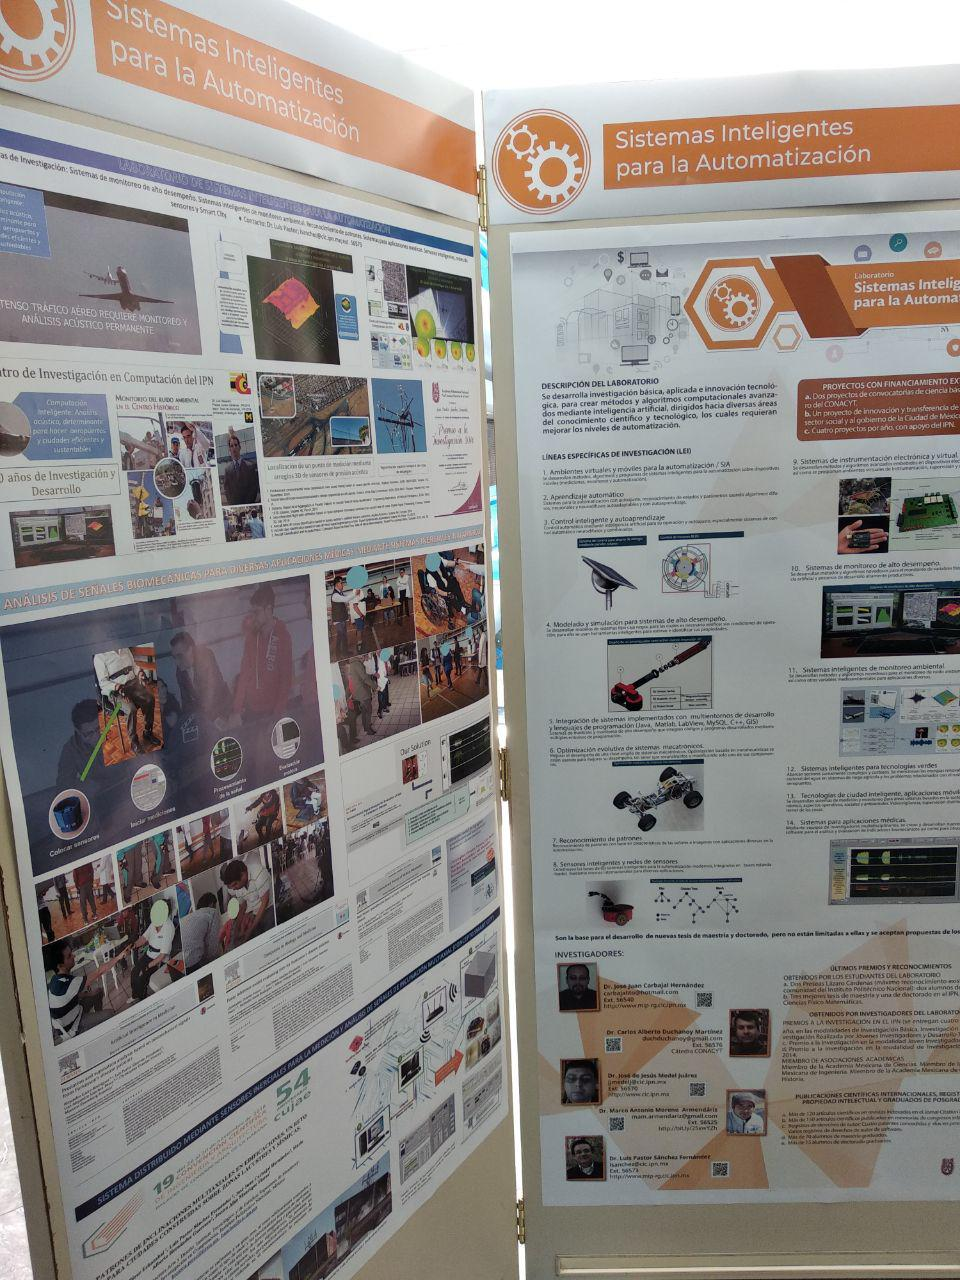
\includegraphics[scale = 0.4]{images/sismo2}
\end{figure}

\subsection*{Análisis de Rutas y Procesamiento de Lenguaje Natural}
Una exposición muy interesante donde nos explicaron dos proyectos.
El primer proyecto trataba de un análisis del transporte público de la Ciudad de México, en el cual se recababa información de estaciones y rutas de los distintos tipos de transporte. Al analizar las rutas y estaciones se puede realizar un mapa de calor que permite observar en que punto de la ciudad se concentra la mayor cantidad de tráfico de usuarios. \\

Este proyecto puede apoyar al gobierno de la ciudad en la toma de desiciones relacionadas con la creación de nuevas líneas y rutas de transporte.\\

\begin{figure}[H]
	\centering
	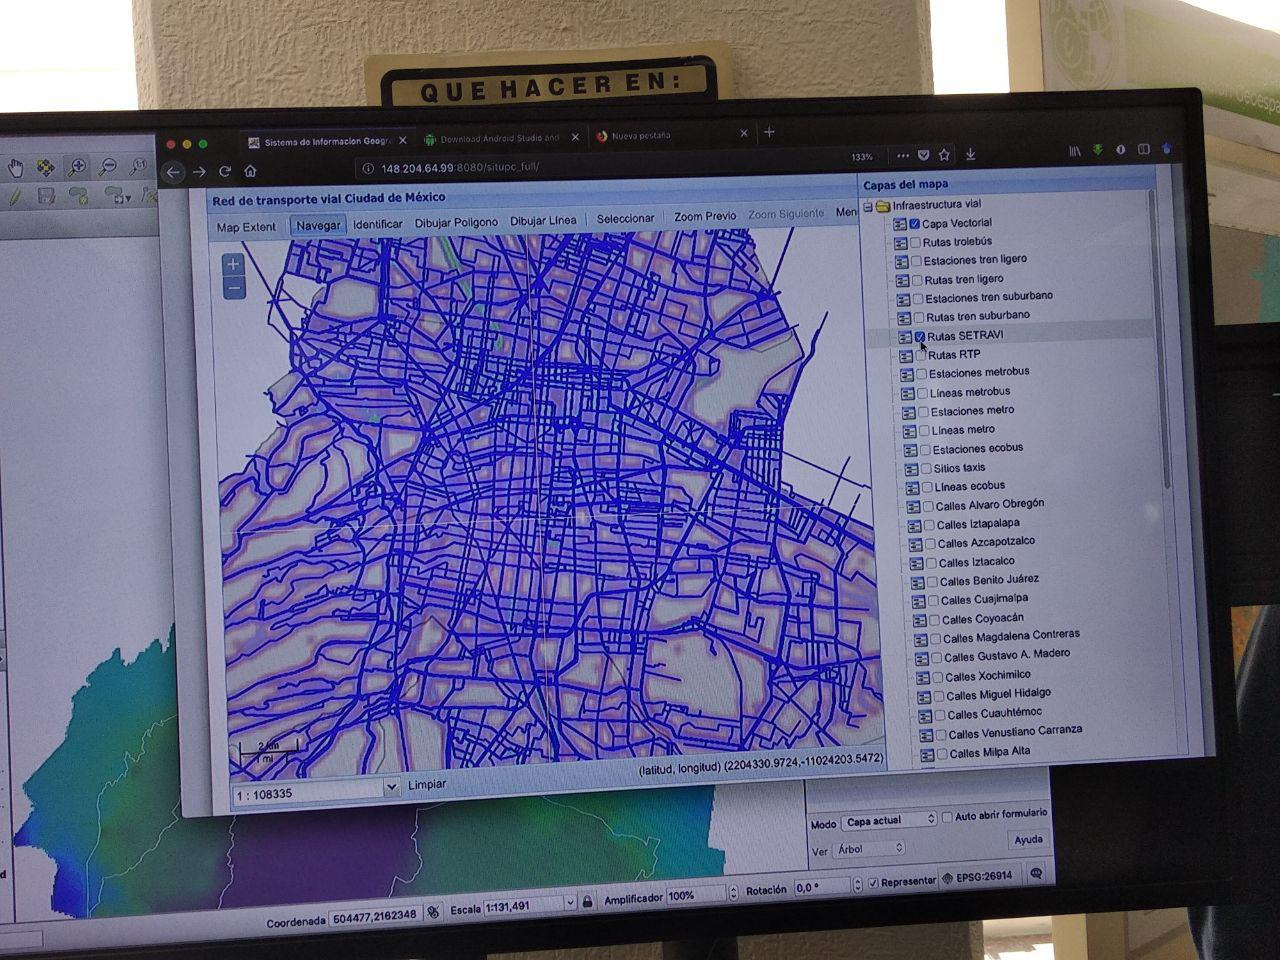
\includegraphics[scale = 0.4]{images/mapa}
\end{figure}

\begin{figure}[H]
	\centering
	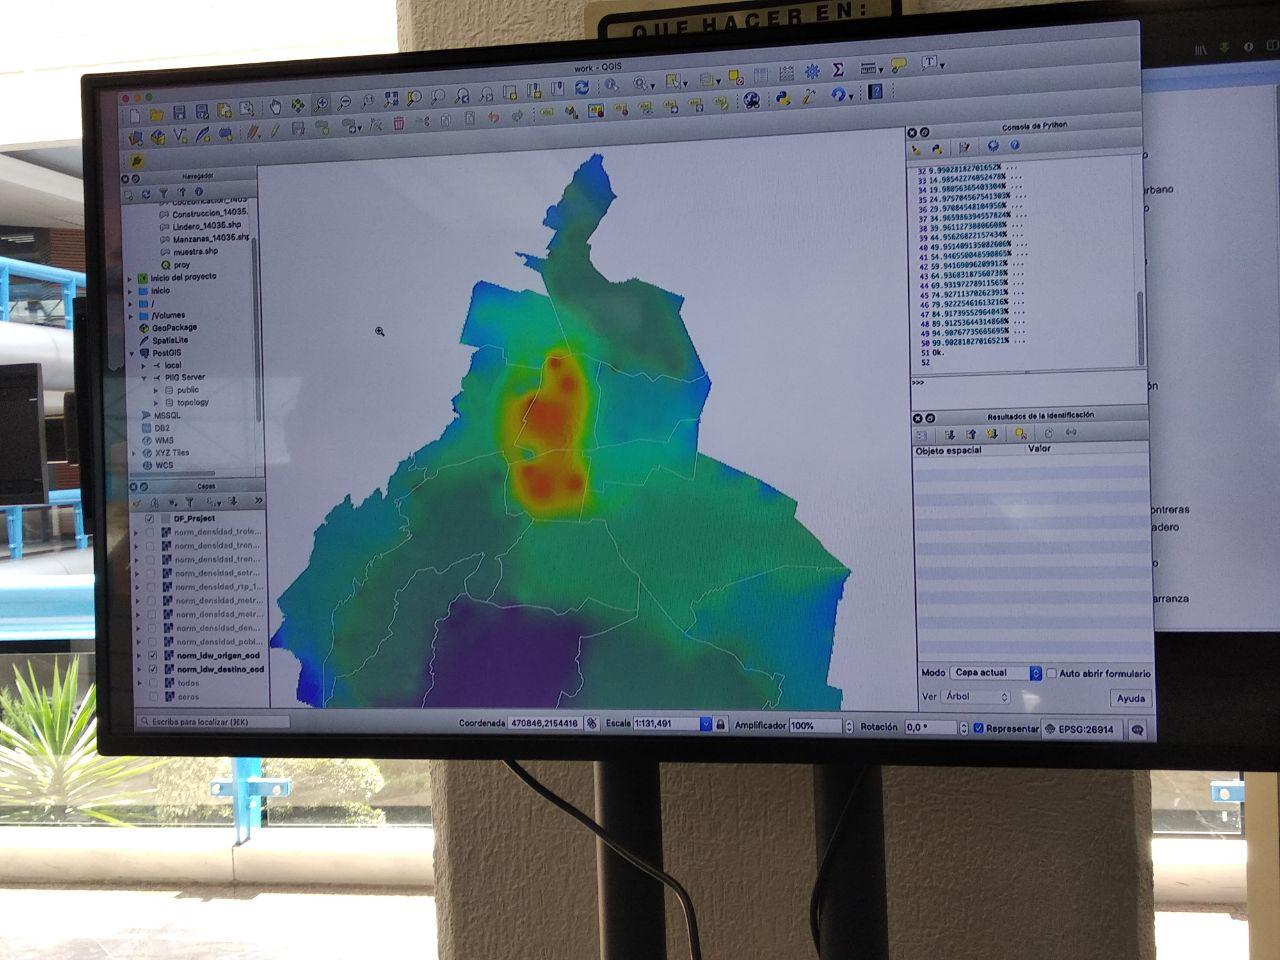
\includegraphics[scale = 0.4]{images/hot}
\end{figure}

El segundo proyecto se trataba de reconocimiento de lenguaje natural, aunque estaba en su etapa inicial, se presentaba la relación de sinónimos mediante grafos. El fin del proyecto a futuro es analizar las publicaciones en redes sociales relacionadas con delincuencia, y mediante el procesamiento del lenguaje natural realizar un mapa de calor que permita identificar las zonas de mayor actividad delictiva.

\begin{figure}[H]
	\centering
	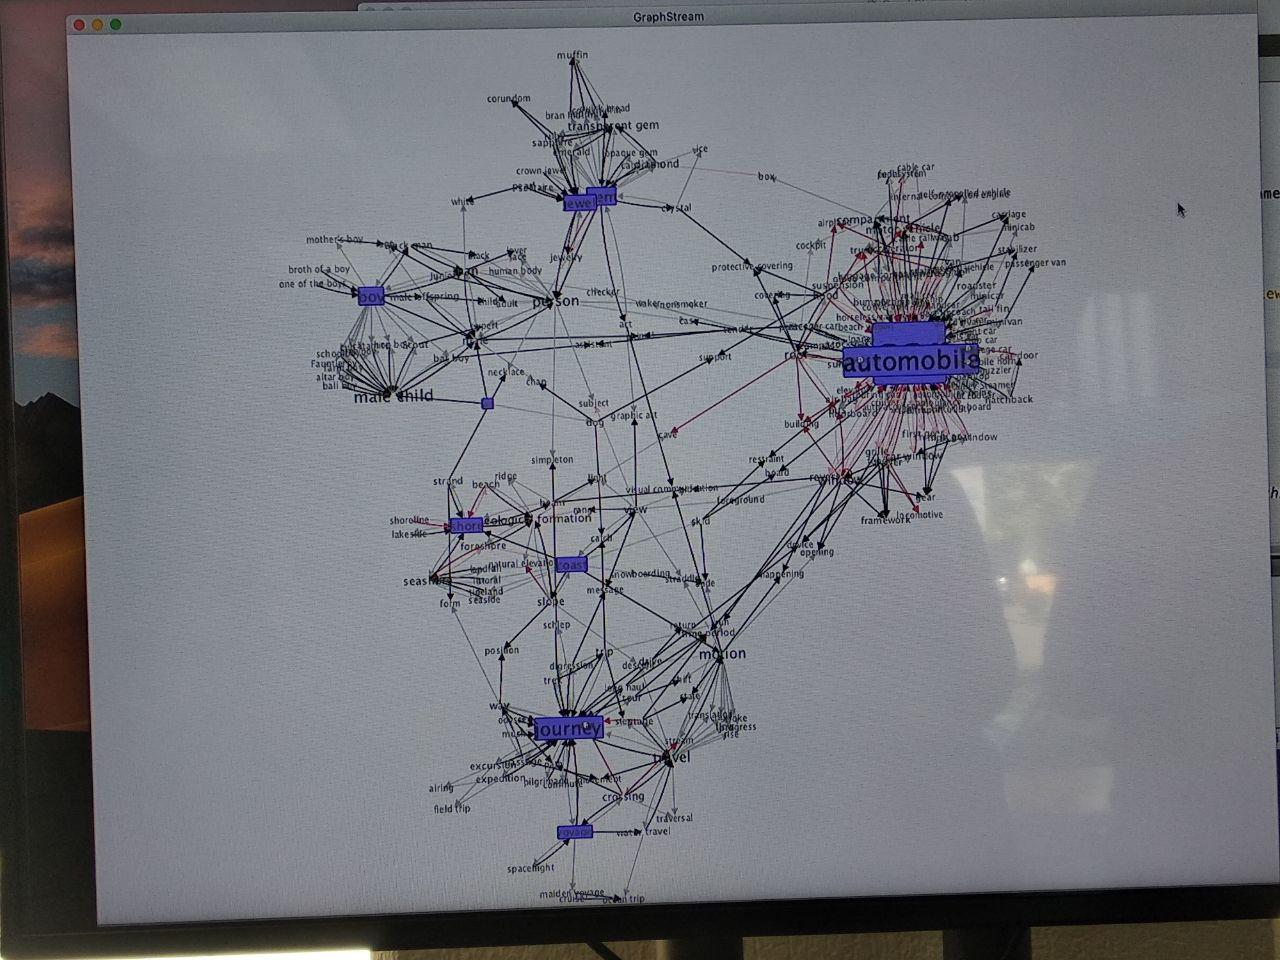
\includegraphics[scale = 0.4]{images/pln}
\end{figure}

\subsection*{Ciencia de Datos y Tecnología de Software}

En este laboratorio se está trabajando en distintos proyectos, por ejemplo:
\begin{itemize}
	\item \textbf{Sistema de Análisis de Movilidad individual (SAM)}: Es una apliación web enriquecida para la visualización de datos históricos que publica el Sistema de Bicicleta Pública de la CDMX.
	\item \textbf{RieSis}: Es una aplicación para apoyar la atención de los estragos provocados por un terremoto de gran magnitud, en una zona densamente poblada.
	\item \textbf{Noti-Explorer}: Es el prototipo de una herramienta para el análisis textual de noticias publicadas en diversos periódicos de Internet. El sistema desarrolla un análisis exhaustivo de las noticias almacenadas desde 2016.
\end{itemize}

\begin{figure}[H]
	\centering
	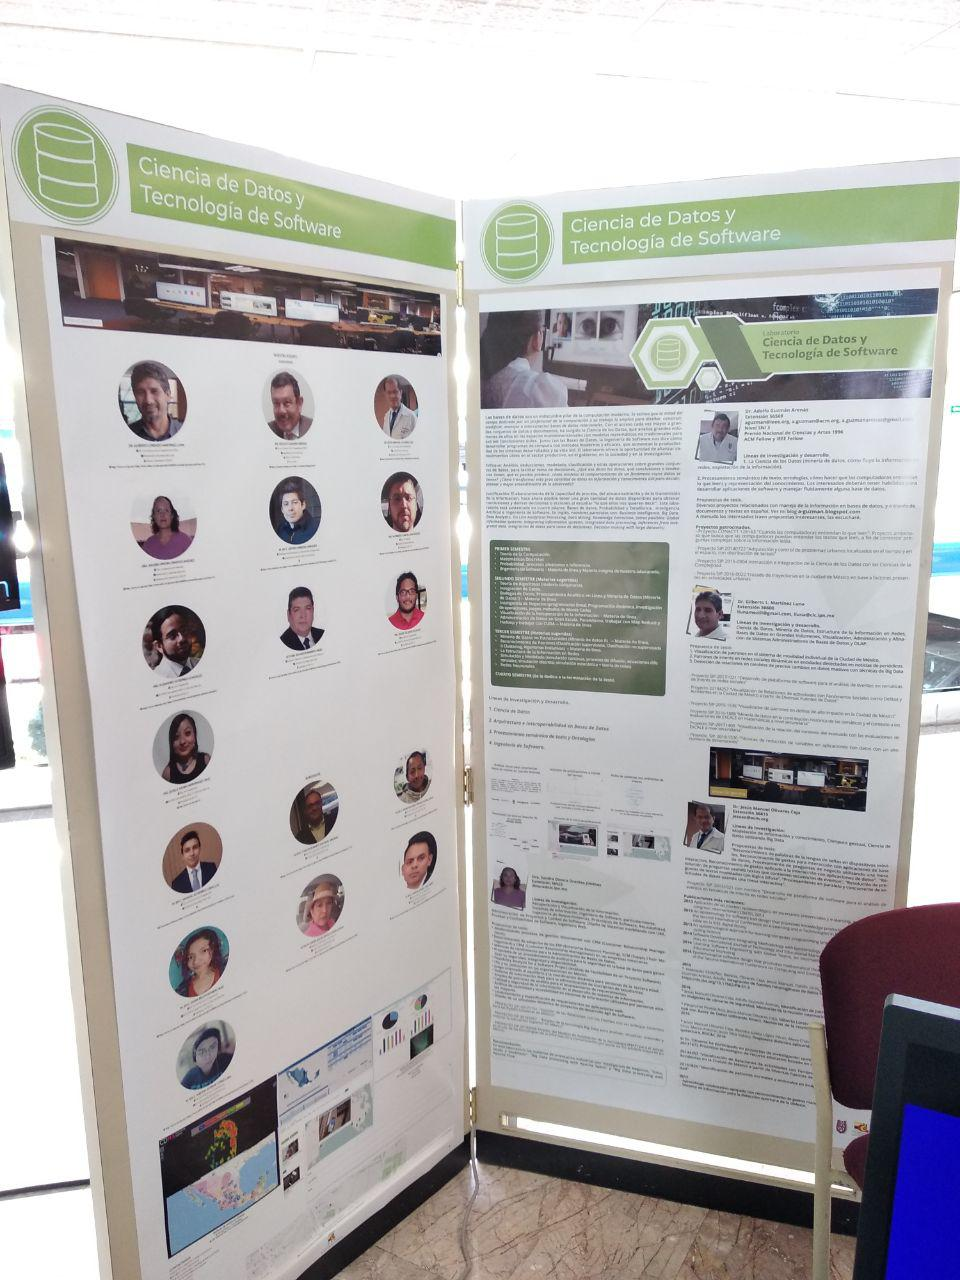
\includegraphics[scale = 0.4]{images/data}
\end{figure}

\end{document}


